%%%%%%%%%%%%%%%%%%%%%%% file template.tex %%%%%%%%%%%%%%%%%%%%%%%%%
%
% This is a general template file for the LaTeX package SVJour3
% for Springer journals.          Springer Heidelberg 2010/09/16
%
% Copy it to a new file with a new name and use it as the basis
% for your article. Delete % signs as needed.
%
% This template includes a few options for different layouts and
% content for various journals. Please consult a previous issue of
% your journal as needed.
%
%%%%%%%%%%%%%%%%%%%%%%%%%%%%%%%%%%%%%%%%%%%%%%%%%%%%%%%%%%%%%%%%%%%
%
% First comes an example EPS file -- just ignore it and
% proceed on the \documentclass line
% your LaTeX will extract the file if required
\begin{filecontents*}{example.eps}
%!PS-Adobe-3.0 EPSF-3.0
%%BoundingBox: 19 19 221 221
%%CreationDate: Mon Sep 29 1997
%%Creator: programmed by hand (JK)
%%EndComments
gsave
newpath
  20 20 moveto
  20 220 lineto
  220 220 lineto
  220 20 lineto
closepath
2 setlinewidth
gsave
  .4 setgray fill
grestore
stroke
grestore
\end{filecontents*}
%
\RequirePackage{fix-cm}
%
%\documentclass{svjour3}                     % onecolumn (standard format)
%\documentclass[smallcondensed]{svjour3}     % onecolumn (ditto)
\documentclass[smallextended]{svjour3}       % onecolumn (second format)
%\documentclass[twocolumn]{svjour3}          % twocolumn
%
\smartqed  % flush right qed marks, e.g. at end of proof
%
% \usepackage{mathptmx}      % use Times fonts if available on your TeX system
%
% insert here the call for the packages your document requires
%\usepackage{latexsym}
% etc.
%
% please place your own definitions here and don't use \def but
% \newcommand{}{}
%
% Insert the name of "your journal" with
% \journalname{myjournal}

\usepackage{calc}
\usepackage{amssymb}
\usepackage{amstext}
\usepackage{amsmath}
\usepackage{color, colortbl}

\usepackage{xcolor} 

\usepackage[final,pdftex]{graphicx}
        \pdfcompresslevel=9
        \DeclareGraphicsExtensions{.png} 

\usepackage{chngcntr}
\usepackage{epsfig} 
\usepackage{url}
 
\usepackage{ifthen} 
\usepackage{amssymb}
 
\usepackage{float} 

\newboolean{showcomments}
\setboolean{showcomments}{false} % toggle to show or hide comments
\ifthenelse{\boolean{showcomments}}
  {\newcommand{\nb}[2]{
    \fcolorbox{gray}{yellow}{\bfseries\sffamily\scriptsize#1}  
    {$\blacktriangleright$#2$\blacktriangleleft$}
   }
   \newcommand{\version}{\emph{\scriptsize$-$working$-$}}
  } 
  {\newcommand{\nb}[2]{}
   \newcommand{\version}{}
  } 

\usepackage[linewidth=1pt]{mdframed}
\usepackage{lipsum}  

% for comments
\newcommand\levi[1]{\nb{Levi}{\textcolor{teal}{#1}}}
\newcommand\moussa[1]{\nb{Moussa}{\textcolor{blue}{#1}}}
\newcommand\adrien[1]{\nb{Adrien}{\textcolor{red}{#1}}}

\usepackage[font={small}]{caption, subfig}

% 
\begin{document}

\title{Process-Aware Model-Driven Development Environments}
%\subtitle{Do you have a subtitle?\\ If so, write it here}

%\titlerunning{Short form of title}        % if too long for running head

\author{First Author         \and
        Second Author %etc.
}

%\authorrunning{Short form of author list} % if too long for running head

\institute{F. Author \at
              first address \\
              Tel.: +123-45-678910\\
              Fax: +123-45-678910\\
              \email{fauthor@example.com}           %  \\
%             \emph{Present address:} of F. Author  %  if needed
           \and
           S. Author \at
              second address
}

\date{Received: date / Accepted: date}
% The correct dates will be entered by the editor


\maketitle

\begin{abstract}
Due to recent advances in Domain Specific Language (DSL) workbenches,
it has become possible to build model-driven development environments
as sets of individual DSLs that get composed for a specific purpose. In
this paper we explore how model-driven development environments can become
process-aware, to assist the user when building a model. We offer an
explanation to our ideas at three levels of abstraction: 1) the meta-meta level,
where brick DSLs are built using the Meta-Programming System (MPS) workbench;
2) the meta level, where brick DSLs are assembled into frameworks that
are further tailored for particular modelling scenarios through the introduction
of an explicit process for model construction; and 3) the model level, where
models are built through progressive tool-guided refinements and automated
steps based on the process introduced at the meta level. We exemplify our
approach by providing the main highlights of the ongoing development of a
model-driven requirements gathering environment for our industrial partners.
\levi{abstract from workshop paper, needs to be rewritten}
\keywords{First keyword \and Second keyword \and More}
% \PACS{PACS code1 \and PACS code2 \and more}
% \subclass{MSC code1 \and MSC code2 \and more}
\end{abstract}

\section{Introduction}

Introduce the problem statement here, something along the following
lines: 

\begin{itemize}
  \item How do we customize a Model-Driven Development environment in order to
  support a given modelling process.
  \item The process should be of an advisory nature and minimally invasive
  regarding the modelling experience.
\end{itemize} 

\section{A conceptual frame for building Process-Aware Model-Driven Development
environments}
\subsection{Variability for customizing MDD environments}

\begin{figure}[h]
   \begin{center}
     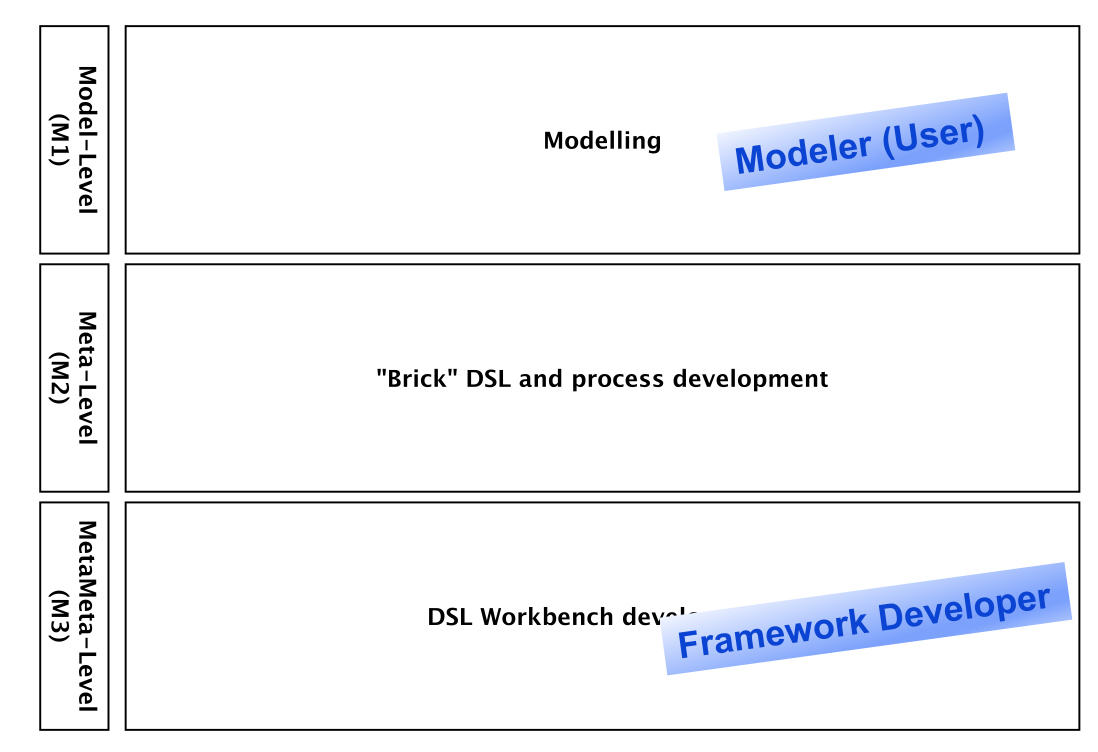
\includegraphics[width=1\columnwidth]{figures/frame.png}
     \caption{Overview of the MDD Environment Stack}
     \label{fig:frame}
   \end{center}
 \end{figure}
 
 
 \begin{figure}[h]
   \begin{center}
     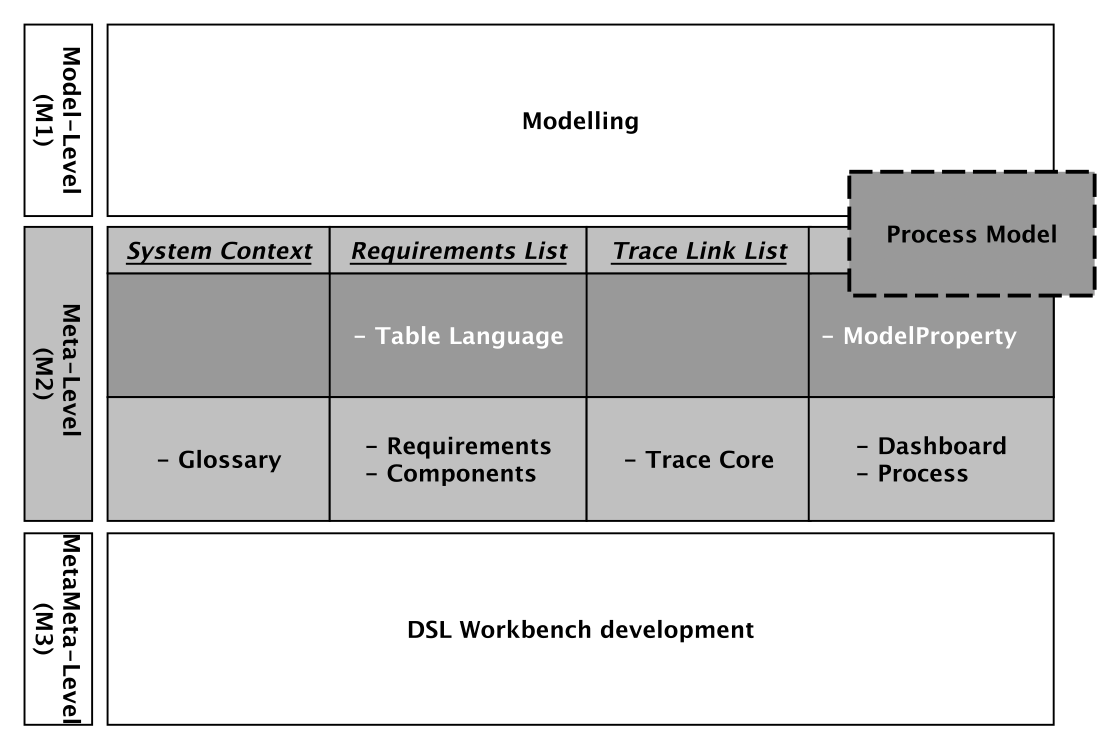
\includegraphics[width=1\columnwidth]{figures/frame_detailed.png}
     \caption{Customizing the MDD Environment}
     \label{fig:frame}
   \end{center}
 \end{figure}
 
 \subsection{Engineering roles in the customization}

\section{Case Studies: The MPS and the AutoFOCUS MDD Environments}
\subsection{MPS and AF3}
\label{sec:mps}
The metameta level (M3, in MOF terms) is where the bricks for our approach are
built. These bricks consist of Domain Specific Languages, defined in the MPS
(Meta Programming System)~\cite{mps} framework. MPS is a stable and
industrially-proven projectional meta-editor. Being a meta-editor, MPS provides edition
capabilities at the meta-levels we need for our approach, in particular M2 and
M1. It uniformly integrates language and editor design capabilities, together
with code generation tools and in-built correct-by-construction tactics such as meta-model
conformance, syntax highlighting, auto-completion or type checking.  
MPS is developed by JetBrains, which assumes the role of \emph{framework
developer}. 

Throughout this paper we will often use vocabulary that is close to that used in
the MPS world in order to remain aligned with the technical aspects of our
work. In particular, the following terms are recurrently used in what follows:

\begin{itemize}
  \item \emph{Language}: an MPS language includes a metamodel, in the classical
  EMF sense. It additionally includes one or more editors for its metamodel,
  which provide concrete syntax. Other aspects of a language
  can be defined and custom new aspects can be
  built by the MPS user (see~\cite{mps} for details).
  \item \emph{Solution}: MPS solutions are projects where users can import
  MPS languages and create their models using those languages.
  \item \emph{Concept}: the MPS equivalent of metamodel class.
  \item \emph{Concept / language instance}: concepts can be instantiated, in
  the same way metamodel classes can. We will also sometimes write
  \emph{language instance} to refer to an instance of the \emph{root} concept of
  an MPS language.
  \item \emph{Intentions}: arbitrary actions attached to concepts of a
  language. Those actions can be launched by the user when the
  focus of the editor is on objects which are instances of those concepts.
  \item \textsf{BaseLanguage Java}: most of MPS' complex language operations are
  coded using the predefined \textsf{BaseLanguage} MPS language, a projectional
  replica of Java enriched with MPS-specific constructs.
  \item \emph{Language composition}:  Reference or containment relations can exist between instances of
  concepts of different languages, which is the primary language composition
  mechanism in MPS. Additionally, an MPS model can contain instances of concepts
  belonging to many languages (not necessarily referring to each other), which
  provides an additional means for language composition.
\end{itemize}

% At this level we had to extend the existing MPS framework with languages to
% define \emph{flow} and a \emph{dashboard}. Additionally, we have provided
% extension points to give the user the possibility to define her own constraints
% that can be used to direct the flow of edition of the composed model.


\subsection{Language stacks in MPS and AF3}

\subsection{Adding guidance to both environments}


\section{Aplication to practice}
%!TEX root = ../paper.tex

\subsection{\doone\ in \afthree}

The \doone\ standard~\cite{do178c} is the primary document by which the certification authorities approve all commercial software-based aerospace systems.
It requires a thorough definition and documentation of the software development process. 
The base set of required documentation includes requirements standard, design standard and traceability.
The \dothree\ standard supplements \doone\ with model-based development guidance.
Both standards define what needs to be done (the objectives that the project must fulfill), but they do not specify how to do so (they do not define a process) .
It is up to the process engineer of each project to define the actual process and document how objectives are achieved.
In this section we describe one such a process and show how it can be implemented in \afthree.
The process guides the requirement engineer and architect to generate requirements and their corresponding design to fulfill some of the standards imposed by \doone\ and \dothree.

Requirements standards required by \doone\ normally impose that information about requirements (ID, name, description, rationale, author, etc) is complete.
Traceability requires that every HLR is related to a SRs.
Once requirements are completed, they need to be reviewed and approved by someone which did not participate in their development. 
The latter guarantees verification independence~\cite{cast26} which must be clearly documented.
According to \dothree, artifacts and their communication channels should have meaningful names, ports should have a type and a range, etc.
Traceability also requires that every artifact in the design shall be traced to a HLR.

We show how the objectives mentioned above can be achieved following our proposed development process.
Objectives are implemented in \afthree\ using constraints.
The first objective is to add requirements to the project. 
Once this is done, two objectives become possible and can be performed in any order. 
\emph{Requirements information complete} assures that the ID, name, description, rationale, author and source (SR from where this requirement is derived) fields are completed. 
The latter defines traces between HLRs and SRs.
\emph{Requirements have an unique aspect} guides the engineer to refine a requirement when it focus on more than a particular aspect.
Consider the following requirement: `\emph{the value of output $o_1$ is the value of input $i_1$ plus 1 and should be computed in less than 5 time units}'.
This requirement contains a functional aspect (how to compute the value of $o_1$) and a timing aspect (what the performance of the computation should be).
Since they refer to different aspects, it is good practice to have both as separated requirements.
The proposed process guides the user to do so.

\subsection{IETS3 in MPS}

\subsection{Assurance cases in AF3}
 

\section{Implementation}
\subsection{Implementation in MPS}

\subsection{Implementation in AutoFOCUS}

\subsection{Lessons learned}

\section{Discussion}

\section{Conclusion} 

\section*{Acknowledgements}
The work presented in this paper was developed \ldots

\bibliographystyle{abbrv}
\bibliography{bibliography}

\end{document}
% end of file template.tex

